%% Copernicus Publications Manuscript Preparation Template for LaTeX Submissions
%% ---------------------------------
%% This template should be used for copernicus.cls
%% The class file and some style files are bundled in the Copernicus Latex Package, which can be downloaded from the different journal webpages.
%% For further assistance please contact Copernicus Publications at: production@copernicus.org
%% https://publications.copernicus.org/for_authors/manuscript_preparation.html


%% Please use the following documentclass and journal abbreviations for preprints and final revised papers.

%% 2-column papers and preprints
\RequirePackage[2020/02/02]{latexrelease}
\documentclass[esurf, manuscript]{copernicus}
%\documentclass[esurf]{copernicus}

%% Journal abbreviations (please use the same for preprints and final revised papers)


% Advances in Geosciences (adgeo)
% Advances in Radio Science (ars)
% Advances in Science and Research (asr)
% Advances in Statistical Climatology, Meteorology and Oceanography (ascmo)
% Annales Geophysicae (angeo)
% Archives Animal Breeding (aab)
% ASTRA Proceedings (ap)
% Atmospheric Chemistry and Physics (acp)
% Atmospheric Measurement Techniques (amt)
% Biogeosciences (bg)
% Climate of the Past (cp)
% DEUQUA Special Publications (deuquasp)
% Drinking Water Engineering and Science (dwes)
% Earth Surface Dynamics (esurf)
% Earth System Dynamics (esd)
% Earth System Science Data (essd)
% E&G Quaternary Science Journal (egqsj)
% European Journal of Mineralogy (ejm)
% Fossil Record (fr)
% Geochronology (gchron)
% Geographica Helvetica (gh)
% Geoscience Communication (gc)
% Geoscientific Instrumentation, Methods and Data Systems (gi)
% Geoscientific Model Development (gmd)
% History of Geo- and Space Sciences (hgss)
% Hydrology and Earth System Sciences (hess)
% Journal of Bone and Joint Infection (jbji)
% Journal of Micropalaeontology (jm)
% Journal of Sensors and Sensor Systems (jsss)
% Magnetic Resonance (mr)
% Mechanical Sciences (ms)
% Natural Hazards and Earth System Sciences (nhess)
% Nonlinear Processes in Geophysics (npg)
% Ocean Science (os)
% Primate Biology (pb)
% Proceedings of the International Association of Hydrological Sciences (piahs)
% Scientific Drilling (sd)
% SOIL (soil)
% Solid Earth (se)
% The Cryosphere (tc)
% Weather and Climate Dynamics (wcd)
% Web Ecology (we)
% Wind Energy Science (wes)


%% \usepackage commands included in the copernicus.cls:
%\usepackage[german, english]{babel}
%\usepackage{tabularx}
%\usepackage{cancel}
%\usepackage{multirow}
%\usepackage{supertabular}
%\usepackage{algorithmic}
%\usepackage{algorithm}
%\usepackage{amsthm}
%\usepackage{float}
%\usepackage{subfig}
%\usepackage{rotating}

\begin{document}

\title{Inverse modeling of turbidity currents using artificial neural network: verification for field application}

% \Author[affil]{given_name}{surname}

\Author[1]{Hajime}{Naruse}

\affil[1]{Graduate School of Science, Kyoto University, Kitashirakawa Oiwakecho, Sakyo-ku, Kyoto, 606-8502 Japan}

%% The [] brackets identify the author with the corresponding affiliation. 1, 2, 3, etc. should be inserted.

%% If an author is deceased, please mark the respective author name(s) with a dagger, e.g. "\Author[2,$\dag$]{Anton}{Aman}", and add a further "\affil[$\dag$]{deceased, 1 July 2019}".

%% If authors contributed equally, please mark the respective author names with an asterisk, e.g. "\Author[2,*]{Anton}{Aman}" and "\Author[3,*]{Bradley}{Bman}" and add a further affiliation: "\affil[*]{These authors contributed equally to this work.}".


\correspondence{Hajime Naruse (naruse@kueps.kyoto-u.ac.jp)}

\runningtitle{Inverse modeling of turbidity currents by neural network}

\runningauthor{Hajime Naruse}





\received{}
\pubdiscuss{} %% only important for two-stage journals
\revised{}
\accepted{}
\published{}

%% These dates will be inserted by Copernicus Publications during the typesetting process.


\firstpage{1}

\maketitle

\begin{abstract}
%#!platex DeepLearningTurbidite.tex

  Although in situ measurements observed on modern frequently occurring turbidity currents have been performed, the flow characteristics of turbidity currents that occur only once every hundreds of years and deposit turbidites over a large area have not yet been elucidated. In this study, we propose a method for estimating the paleo-hydraulic conditions of turbidity currents from ancient turbidites by using machine learning. In this method, we hypothesize that turbidity currents result from suspended sediment clouds that flow down a steep slope in a submarine canyon and into a gently sloping basin plain. Using inverse modeling, we reconstruct seven model input parameters including the initial flow depth, the sediment concentration and the basin slope. A reasonable number (3,500) of repetition of numerical simulation using one-dimensional layer-averaged model under various input parameters generates a dataset of the characteristic features of turbidites. This artificial dataset is then used for supervised training of a deep learning neural network (NN) to produce an inverse model capable of estimating paleo-hydraulic conditions from data of the ancient turbidites. The performance of the inverse model is tested using independently generated datasets. Consequently, the NN successfully reconstructs the flow conditions of the test datasets. In addition, the proposed inverse model is quite robust to random errors in the input data. Judging from the results of subsampling tests, inversion of turbidity currents can be conducted if an individual turbidite can be correlated over 10 km at approximately 1 km intervals. These results suggest that the proposed method can sufficiently analyze field-scale turbidity currents.
\end{abstract}


\copyrightstatement{}


\introduction  %% \introduction[modified heading if necessary]
%#!pdflatex Naruse_Esurf_2020.tex

Turbidity currents are sediment-laden density flows that occur intermittently in deep sea environments \citep{Talling2014}. Turbidity currents are the main drivers of mass circulation processes in deep sea environments. In fact, estimating the flux of organic carbon transported and buried by turbidity currents is particularly necessary to understand the carbon cycle processes \citep{Buscail1997,Heussner1999}. In addition, the deposits of turbidity currents, i.e., turbidites, form a submarine fans on the sea floor, which may function as large-scale hydrocarbon reservoirs \citep{Kendrick1998,Yoneda2015}, and are thus economically essential.

Through recent development of observational instruments, the velocity and flow depth of deep-sea currents can be measured directly \citep{Clarke2016}. Consequently, numerous records of turbidity currents have been reported at locations such as Squamish Bay, Canada \citep{Clarke2016}, Monterey canyon offshore California \citep{xu2004insitu,xu2010normalized,Paull2018}, and the Congo Submarine Channel \citep{vangriesheim2009turbidity,azpiroz2017newly}. Surprisingly, these records revealed that turbidity currents occurs almost monthly in the modern submarine environments \citep{Paull2018}. On the contrary, the record in Squamish indicated seven events even in one day. However, the turbidites observed in outcrops and cores are deposited at intervals of 500-1000 years or longer. For example, \citet{Ishihara1997} investigated the deposits of the fore-arc basin (the Pliocene Awa Group) and reported that turbidite beds were deposited approximately once every 1200-1300 years. \citet{Clare2014} analyzed turbidites in the western Mediterranean Sea, off the northwest coast of Africa and the Apennines, and found that they were deposited with a frequency of about 1,400-36,000 years in all regions. In contrast to these geologic records, the recent field observations show that turbidity currents are not a rare event.

What caused the difference in observed frequency of modern turbidity currents compared with the records of ancient turbidites? One of the possibilities is that most of the turbidity currents observed in the present day may be very small in magnitude or are diluted, and leave little or no deposits in large areas. If this is the case, turbidites of several tens of centimeters thick observed in geologic records can be interpreted as deposits of extraordinarily large-scale events that occurred once every several hundred years. This hypothesis implies that turbidites in the strata resulted from low-frequency but very high-risk events such as large tsunamis and earthquakes \citep{Goldfinger2003a}. In this case, we would have to assume that the velocity and concentration of turbidity currents obtained from in-situ observations are quite different from those of turbidite-forming currents in strata. Another possibility is that the areas where turbidity currents have been measured experienced very special conditions and that the frequency of turbidity currents will be significantly reduced even in those areas over long time scales. It is very difficult to determine which of these hypotheses is correct at this time because typical hydraulic conditions under which ancient turbidites were deposited have not been well understood. Although the characteristics of turbidity currents in natural environments have been elucidated rapidly through recent \textit{in situ} observations of flow properties \citep{Paull2018}, the flow characteristics of turbidity currents that form actual submarine fans remain unknown.

The inverse analysis of turbidites in strata may fill the gap between the observations of turbidity currents and the geologic field observations of ancient turbidites. The reconstruction of past conditions by inverse analysis has been a major tool in several research fields including sedimentology and geomorphology. For example, several studies have reconstructed the magnitudes of past tsunamis from tsunami deposits \citep{Jaffe2007, Naruse2017, Mitra2020a}, and \citet{Rossano1996} estimated the behavior of pyroclastic flows using inverse analysis. If the hydraulic conditions of turbidity currents, such as velocity and concentration from turbidites can be reconstructed, it should be possible to verify whether turbidite beds in geologic records were deposited from flows of different scales or not by comparing the reconstructed values with the \textit{in situ} observations. 

However, no practical methodology for the inverse analysis of turbidity currents applicable on a field scale has yet been established. Early attempts to obtain hydraulic parameters of turbidity currents were based on the grain-size distribution of turbidites \citep{SCHEIDEGGER1965,vanTassell1981,Bowen1984,Komar1985,Kubo1995} or on sedimentary structures \citep{Harms1960,Walker1965,allen1982sedimentary,Komar1985,allen1991bouma,baas2000duration}. The estimation of hydraulic conditions for turbidity currents based on grain size assumed that the flow is close to the criteria of suspension or the auto-suspension \citep{Komar1985}, but it has been emphasized that this assumption is highly problematic and leads to significantly different results compared with the actual hydraulic conditions for turbidity currents \citep{Hiscott1994}. Although the methods based on sedimentary structures can provide rough estimates of the conditions of a turbidity current, assumptions regarding the thickness of the flow are required \citep{Ohata2017}. 

To obtain reasonable flow characteristics from turbidites, inverse analysis using a numerical model should be performed. \citet{Falcini2009} proposed a method for predicting the hydraulic conditions of turbidity currents from ancient turbidites and applied it to the Laga Formation in the Central Apennines, Italy. Their steady-state model was largely simplified to obtain an analytical solution of the model. However, most of the ancient turbidites are characterized by graded bedding \citep{Bouma1962}, which suggests non-steady waning nature of currents. Therefore, the applicability of this method should be quite limited to non-graded turbidites deposited from long-maintained flows. Conversely, \citet{lesshafft2011towards} applied a direct numerical simulation model for the inversion of turbidite, whose application however to field-scale data is difficult because of the high calculation cost. \citet{Parkinson2017} proposed a method applicable to non-steady field scale flows by using a layer-average model as the forward model, which is potentially applicable to turbidites in outcrops. However, the flow conditions predicted from ancient turbidites were quite unrealistic in their study. They analyzed a turbidite in the Marnoso Arenacea Formation in the Appennine, and gave flow depth of  3950 m or 1.92 mm; both reconstructions are not acceptable as realistic conditions. These extremely large or small estimates may be due to oversimplification in their forward model or failure in the optimization of the input parameters. \citet{Nakao2017} were the first to successfully perform an inverse analysis of turbidites using a general non-steady layer-averaged model. Although their reconstruction of the hydraulic conditions of the turbidity current was reasonable, the computational load of the inverse analysis was high because they used a genetic algorithm for optimization. Thus, they were unable to repeatedly analyze various artificial or field data to test the validity and robustness of their inverse model. In addition, because of the high computational load, modifying their forward model to a more complex one in future would be difficult. These previous attempts suggest that a robust inverse model that can accept a more complex forward model is required to conduct inversion of turbidity currents from turbidites under realistic conditions.

Here, we propose a new methodology using an artificial neural network (NN) for obtaining flow characteristics of turbidity currents from their deposits (Fig. \ref{fig:schematic_diagram_procedures}). NNs are machine learning systems that can be trained to perform very complex functions \citep{HechtNielsen1987}. NNs have been used in a wide range of applications such as classification \citep{Krizhevsky2012} or generative modeling \citep{Sun2018}. In recent years, this method has been widely applied also in the field of earth and planetary sciences \citep{Laloy2018}. Particularly, NNs are a powerful tool for high-dimensional regression of multiple variables with complex distributions \citep{LeCun2015}. In this study, we generate a non-linear regression model to estimate the hydraulic conditions of turbidity currents from the spatial distribution of bed thickness and grain size of turbidites using NN. If the regression is adequate, the NN can be used as an inverse model of turbidity currents. However, there are too few \textit{in situ} measurements of hydraulic conditions of turbidity currents available. Although it is predicted that at least several hundred datasets of hydrological conditions and depositional characteristics are required to train NN, such frequent observation of turbidity currents that occur intermittently on the deep seafloor cannot be expected. Therefore, the method proposed in this study is designed to generate data of deposits from known conditions by numerical calculations of the forward model. In this case, the generation of training data can be completely parallelized, and therefore, any model that incur a high computational load can be implemented as a forward model. 

In this study, we implement a NN-based inverse analysis and examine its effectiveness for turbidites at the field scale. The focus of this study is on rapidly decelerating sedimentary turbidity currents, and normally graded turbidites are considered to be deposited from such decaying flows. This approach was already proved to be effective for the inverse analysis of tsunami deposits \citep{Mitra2020a}. However, the forward model used in their study was based on the assumption of quasi-steady flow, and thus our work is the first time to perform the inverse analysis using a neural network with completely unsteady flow. The success of the inverse analysis for turbidity currents, which exhibit quite different properties from those of tsunamis, would indicate the wide applicability of our inversion framework for event deposits.

\begin{figure}[t]
  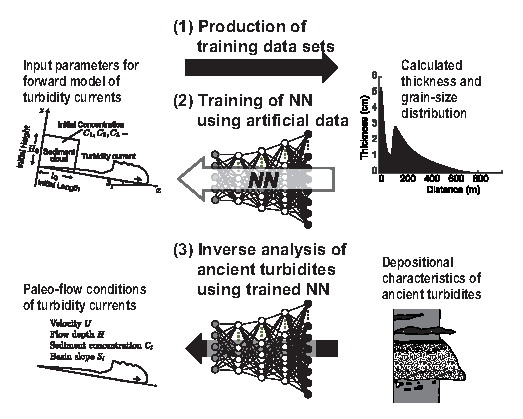
\includegraphics[width=8.3cm]{fig01.eps}
  \caption{Schematic diagram of the inversion process of turbidity currents from deposits. The method is composed of three steps: (1) generation of training data sets by the forward model using random values for model input parameters, (2) trainng of NN based on the artificial data sets, and (3) application of the trained inverse model to unknown field data sets}
  \label{fig:schematic_diagram_procedures}
\end{figure}



%#!pdflatex Naruse_Esurf_2020.tex











\begin{table}[t]
  \caption{Precision and bias of predicted parameters.}
  \begin{tabular}{lrrrrrrr}
    \hline
    {} &  R\textasciicircum 2 &  RMSE &  RMSE (normalized) &   MAE &  MAE (normalized) &  Mean bias &  Mean bias (normalized) \\
    \hline
    Initial height & 0.99 & 18.97 &               8.55 & 14.81 &              5.96 &     -12.93 &                   -0.05 \\
    Initial length & 0.99 & 15.82 &               7.53 & 12.09 &              4.92 &      -2.33 &                   -0.02 \\
    C\_1            & 0.99 &  0.02 &              12.91 &  0.02 &              6.00 &      -0.01 &                   -0.04 \\
    C\_2            & 0.99 &  0.02 &              15.57 &  0.02 &              7.67 &      -0.01 &                   -0.04 \\
    C\_3            & 0.99 &  0.02 &              13.03 &  0.02 &              6.39 &      -0.00 &                   -0.02 \\
    C\_4            & 0.99 &  0.03 &              13.71 &  0.02 &              6.67 &      -0.01 &                   -0.04 \\
    S\_l            & 0.98 &  0.03 &              19.56 &  0.03 &             11.67 &       0.03 &                    0.11 \\
  \hline
    \end{tabular}
  \label{table:bias_errors}
\end{table}




%#!pdflatex Naruse_Esurf_2020.tex

\section{Forward model description}

Here we describe the formulation of the forward model used for producing training datasets for the inverse model (Fig. \ref{fig:model_explanation}). This model is based on the model developed by \citet{kostic2006response}, which predicts the behavior of surge-type turbidity currents, but we modified it to consider sediment transport and deposition of multiple grain-size classes. The initial setting of the flows was set to be the lock-exchange condition, which assumes that the collapse of a rectangular-shaped cloud of sediment suspension produces a turbidity current.

\begin{figure*}[t]
  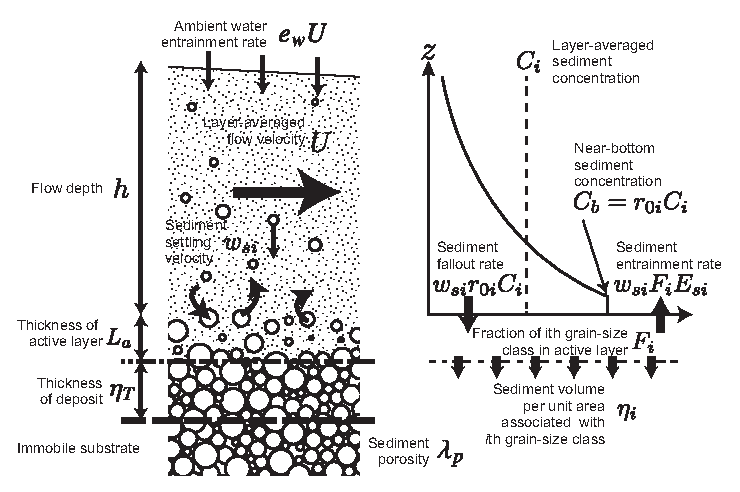
\includegraphics[width=12cm]{fig02.eps}
  \caption{Explanation of model parameters. The turbidity current exchanges suspended sediment with the active layer ($L_{a}$ in thickness) on the top of the deposit ($\eta_T$ in thickness) by settling and entrainment. The volumetric rate of settling of the $i$th grain-size class of sediment is calculated from the basal sediment concentration $r_{0} C_i$ multiplied by the sediment settling velocity $w_{s}{i}$. The sediment entrainment rate from the active layer is $w_{si} F_i e_{si}$, where $F_i$ is the volumetric fraction of the $i$th grain-size class in the active layer and $E_{si}$ is the unit dimensionless rate of sediment entrainment. The time variation of grain-size distribution in the active layer is computed in this model.}
  \label{fig:model_explanation}
\end{figure*}


\subsection{Layer-averaged equations}

Let $t$ and $x$ be the time and bed-attached streamwise coordinates, respectively. Parameters $U$ and $h$ denote the layer-averaged flow velocity and the depth, respectively. The total sediment concentration is $C_T$. Here, we apply the following layer averaged conservation equations of fluid mass, momentum and suspended sediment mass of a turbidity current \citep{parker1986self,kostic2006response}:

\begin{eqnarray}
  \frac{\partial h}{\partial t} + \frac{\partial Uh}{\partial x} & = & e_wU \label{eq:conserv_fluidmass} \\
  \frac{\partial Uh}{\partial t} + \frac{\partial U^2h}{\partial x} & = & R g C_T h S - \frac{Rg}{2}\frac{\partial C_T h^2}{\partial x} - C_f U^{2} \label{eq:conserv_momentum} \\
\frac{\partial C_i h}{\partial t} + \frac{\partial U C_i h}{\partial x} & = & w_{si} (F_i e_{si} - r_0 C_i) \label{eq:conserv_suspensionmass}
\end{eqnarray}

\noindent where $R(=\rho_s/\rho_f - 1)$ is the submerged specific density of the sediment ($\rho_s$ and $\rho_f$ are the densities of the sediment and the fluid), and $g$ is the gravity acceleration. $S$ is the slope, and $C_f$ denotes the friction coefficient. The right-hand side of the fluid mass conservation (Equation \ref{eq:conserv_fluidmass}) considers the entrainment of ambient fluid to the flow, in which the empirical entrainment coefficient $e_w$ is applied. Equation \ref{eq:conserv_suspensionmass} describes the mass conservation of the suspended sediment in the flow, which varies depending on the balance between settling and entrainment of the sediment from and to the active layer. In this model, the grain-size distribution of sediment is discretized to $N$ classes. The parameter $C_i$ denotes the suspended sediment concentration of the $i$th class. The model applies the active layer assumption, in which the grain-size distribution is vertically uniform in the bed surface layer (active layer) that exchanges sediment with suspended load \citep{Hirano1971}. $F_i$ indicates the fraction of the $i$th grain-size class in the active layer. The parameter $w_{si}$ denotes the settling velocity of the sediment particles in the $i$th class, and $r_0$ denotes the ratio of near-bed concentration to the layer-averaged concentration of the suspended sediment.

The mass conservation of the sediment in the active layer and the deposit (historical layer), respectively, takes respectively the form

\begin{eqnarray}
  \frac{\partial \eta_i}{\partial t} & = & \frac{w_{si}}{1-\lambda_p}(r_0 C_i - e_{si} F_i) \label{eq:conserv_bed} \\
\frac{\partial \eta_T}{\partial t} &=& \sum \frac{\partial \eta_i}{\partial t}.
\label{eq:total_exner_equation} \\
\frac{\partial F_i}{\partial t} + \frac{F_i}{L_a}\frac{\partial \eta_T}{\partial t} & = & \frac{w_{si}}{L_a (1 - \lambda_p)}(r_0 C_i - F_i e_{si} ). \label{eq:conserv_activelayer}
\end{eqnarray}

\noindent where $\eta_i$ denotes the volume per unit area of the $i$th grain size class, and $\eta_T$ is the total thickness of the deposit. $L_a$ denotes the thickness of the active layer, which is assumed to be constant, for simplicity. The parameter $\lambda_p$ denotes porosity of the active layer and the deposit (0.4 in this study), and $e_{si}$ is an empirical coefficient for sediment entrainment of the $i$th class from the active layer. Equation \ref{eq:conserv_bed} describes the mass conservation of the $i$th class sediment in the bed, and rate of the bed aggradation is obtained by summation of accumulation rates of all grain-size classes (Equation \ref{eq:total_exner_equation}). Equation \ref{eq:conserv_activelayer} considers the temporal development of the grain size distribution in the active layer, where the time development of the total bed thickness $\eta_T$ is obtained by summation of the right-hand side of Equation \ref{eq:conserv_bed} for all grain-size classes.

To solve the Equations \ref{eq:conserv_fluidmass}--\ref{eq:conserv_activelayer}, empirical relations are required for the parameters: $w_{si}$, $r_0$, $C_f$, $L_a$, $e_w$, and $e_{si}$. Here we applied the formulation of \citet{dietrich1982settling} for obtaining the settling velocity $w_{si}$. The ratio of near-bed to layer-averaged concentrations $r_0$ and the bed friction coefficient $C_f$ are fixed to be 2.0 and 0.004, for simplicity \citep{Garcia1990}. The active layer thickness $L_a$ is assumed to be constant (0.003 m). Regarding the entrainment coefficients of ambient water and basal sediment $e_w$ and $e_{si}$, we applied formulations proposed by \citet{parker1987experiments} and \citet{garcia1991entrainment} respectively.

For computational efficiency and numerical stability, a deformed grid approach was adopted to solve Equations \ref{eq:conserv_fluidmass}--\ref{eq:conserv_suspensionmass}. In this transformed coordinate, the propagating flow head was fixed at the downstream boundary using a Landau transformation \citep{Crank1984}. The tail of the flow was also fixed at the upstream end of the calculation domain, and thus the grid spacing in the dimensional coordinate space was continuously stretched during calculation, whereas that in dimensionless space remained constant. This scheme was based on \citet{kostic2006response}, and more details regarding the numerical implementation were given by \citet{Nakao2017}.

\subsection{Model input parameters and topographic settings}
In this study, a turbidity current was assumed to occur from a cloud of suspended sediment (height: $H_0$, length $l_0$). The initial flow velocity was set to 0, and the sediment of the $i$th grain-size class was considered to be initially homogeneously distributed in the suspension cloud at the concentration $C_i$ (Fig. \ref{fig:model_input_parameters}). The suspended sediment cloud was located at the upstream end of the calculation domain, where the slope gradient was 0.1. This steep slope extended for 5.0 km and transited to a gently sloping basin plain (gradient is $S_l$) in the downstream region. Total length of calculation domain was 100 km. In summary, the number of initial conditions required for the forward model calculation was three ($H_0$, $l_0$ and $S_l$) plus number of grain-size classes ($C_i$). 

\begin{figure}[t]
  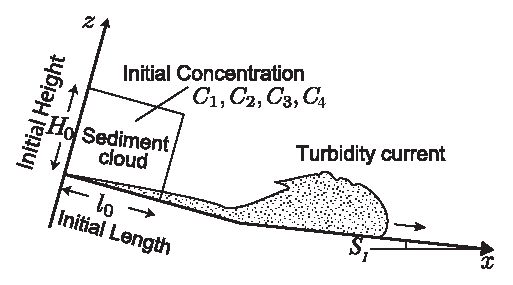
\includegraphics[width=8.3cm]{fig03.eps}
  \caption{Model input parameters. The initial conditions of turbidity current is assumed to be the suspended sediment cloud that is $H_0$ and $l_0$ in height and length, respectively. The initial sediment concentrations $C_1$ to $C_4$ and the basin slope $S_l$ are to be specified for calculation. These seven input parameters are subject to be reconstructed by inverse analysis.}
  \label{fig:model_input_parameters}
\end{figure}


%#!pdflatex Naruse_Esurf_2020.tex

\section{Inverse modeling by deep learning NN}
In this study, numerical simulation of a turbidity current is repeated under various random initial conditions to produce a data set of the characteristic features of turbidites. Then, this artificial dataset of turbidites is used for supervised training of a deep learning NN. The values of the turbidites characteristics, i.e., distribution of volume-per-unit-area of all grain size classes, in the training data set are input to the NN, and the estimated initial conditions (e.g., initial flow height and concentration) of the turbidity current is obtained from the output nodes of NN. The output values of the NN are compared with the true conditions. The optimization of weight coefficients of NN is then conducted to reduce the mean square of the difference between the true conditions and the output values of the NN. If the number of training datasets is sufficiently large, the trained NN should be able to estimate the paleo-hydraulic conditions from the data of the ancient turbidites (Fig. \ref{fig:schematic_diagram_procedures}). In other words, an empirical relationship with numerical results and the model input parameters are explored in this method, and the discovered relationship is used for inverse modeling of turbidity currents. The details of these procedures are described below.

\subsection{Production and preprocessing of training and test data sets for supervised machine learning}

We conducted iterative calculations using the forward model and accumulated data to train and validate the inverse model. To investigate the appropriate amounts of data for training the inverse model, we conducted 500--3500 iteration of the forward model calculations. To verify the performance of the trained model, 300 test data sets were also generated numerically, independent of the training data.

Model input parameters that are subject to inversion are required to produce the training and test data by the forward model calculation (Fig. \ref{fig:model_input_parameters}). In this study, the model inputs are the initial flow height $H_0$, the initial flow length $l_0$, the initial sediment concentration for the $i$th grain size class $C_i$, and the basin slope $S$. These model parameters are generated as uniform random numbers within a certain range, and their range is changed according to the target of the inverse analysis. Since this study is aimed at field-scale analysis, the following ranges are chosen. Both initial depth and length of suspended cloud range from 50 to 600 m. The sediment concentration for each grain size class ranges from 0.01\% to 1.0\%. The number of grain size classes $N$ is four, and the representative grain diameters are 1.5, 2.5, 3.5 and 4.5 phi. The inclination of the basin plain where the turbidites are expected to form ranges from 0 to 1.0\%. 

Each run of the forward model calculation is initiated with the given model input parameters, and is terminated when the flow head reaches the downstream end or sufficiently long time period ($1.2 \times 10^5$ s.) has elapsed. As a result of the calculation, the forward model outputs the volume-per-unit-area of sediment for all grain size classes over the 100 km-long calculation domain. The inverse model estimates the model input parameters from the resultant spatial distribution of the granulometric characteristics of the deposits. However, in natural outcrops, it is unlikely that the entire distribution of the turbidite beds would be exposed. Therefore, we limit the length of the sampling window in the calculation domain, and only the sediment data contained in this window is extracted for both training and testing. The upstream end of the sampling window was set at the transition point between the steep slope and the basin plain (5 km from the upstream end), and the length of the window varies from 1 to 30 km to evaluate the data interval required for the inverse analysis.

Before the model input parameters are input to NN, all values are normalized between 0 and 1 using the following equation:

\begin{equation}
I_{i}^{*} = \frac{I_i - I_{min}}{I_{max} - I_{min}}
\label{eq:normalization}
\end{equation}

\noindent where $I_i^*$ and $I_i$ denote the $i$th normalized and original input parameters, respectively. $I_{\mathrm{max}i}$ and $I_{\mathrm{min}i}$ are the maximum and minimum values used for generating the $i$th input parameter, respectively. This min-max normalization is applied to consider all parameters at equal weights because the range of the initial flow conditions is significantly different between them.

\subsection{Structure of NN}
The artificial NN is used as the inverse model to reconstruct flow conditions from the depositional architecture. We input the spatial distribution of volume-per-unit-area of multiple grain size classes of a turbidite in the NN, which outputs the values of the flow initial conditions and the basin slope. In this study, we use a fully connected NN that has four hidden layers. The volume-per-unit-area of $N$ grain-size classes of sediment deposited on $M$ spatial grids in the sampling window is given to the input nodes of the NN. Thus, the total number of the NN input nodes is $N \times M$. The number of nodes in all hidden layers is set to 2000 in this study. 

The Rectified Linear Unit (ReLU) activation function is adopted for all NN layers \citep{Nair2010, Glorot2011}. The ReLU is the half-wave rectifier $f(z) = \max(z, 0)$. Compared with other smoother non-linearities, such as $\tanh(z)$ or $1/(1+\exp(-z))$, the ReLU typically learns much faster in NN with multiple layers \citep{Glorot2011}, and thus it allows to train a deep supervised network without unsupervised pre-training \citep{LeCun2015}.

The NN is expected to output the model input parameters (i.e., the initial flow conditions and the basin slope), and therefore, the number of nodes in the output layer is equal to the number of input parameters for the forward model, which is seven here (the initial flow length, depth, sediment concentrations and the basin slope).

\subsection{Training the inverse model}
To develop the inverse model, supervised training is conducted using the artificial dataset produced by the forward model calculation. First, the artificial dataset is randomly split into training and validation datasets to detect overfitting during the training process. The ratio of the validation dataset is set to 0.2 so that 80\% of the artificial dataset is used for training. The model input parameters used for producing training and validation sets were regarded as the teacher data to train and evaluate the model.

Methodology applied for training the NN is as follows. The mean squared error (MSE) is adopted as the loss function because the supervised training of NN in this study is classified as a regression problem \citep{Specht1991}, and MSE is a common loss function for regression \citep{Bishop2006,Hastie2009,ShalevShwartz2014}. Before training, all weight coefficients of NN are randomly initialized using the Glorot uniform distribution \citep{Glorot2010}. The backpropagation algorithm \citep{Rumelhart1986} is used to calculate the derivative of this error metric for each connection between the nodes, and the stochastic gradient descent method (SGD) with Nesterov momentum \citep{NESTEROV1983} is used for optimizing the weight coefficients of NN to minimize the difference between the model predictions and the teacher datasets. Other optimization methods, such as AdaGrad \citep{Duchi2011}, RMSprop \citep{Tieleman2012} and AdaDelta \citep{Zeiler2012}, have been tested, but SGD shows the best performance in this case. Dropout regularization \citep{Srivastava2014} is applied for each epoch to reduce overfitting and to improve the generalization ability of the NN. One training epoch, which refers to one cycle through the full training dataset, is repeated until the loss function of the validation dataset converges to a constant value. These methods are all implemented in Python with the library Tensorflow 2.1.0 \citep{Raschka2019}, and the calculations are conducted using GPU NVIDIA GeForce GTX 2080 Super with libraries CUDA 11.0 and CuDNN 7.0.

Several hyperparameters should be specified for the training of NN. Specifically, the dropout rate, the learning rate, the batch size, the number of epochs, and the momentum are adjusted manually after repeated trial and error. To perform an optimization calculation with SGD, the batch size and the learning rate were set to 32 and 0.02, and the value 0.9 was chosen for the momentum. Dropout rate for regularization was 0.5. 

\subsection{Testing the inverse model}

The performance of the inverse model is tested using a set of 300 data that are produced independently of the training and validation datasets. The inversion precision for each model input parameter is evaluated by the root mean square error (RMSE) and the mean absolute error (MAE) of the prediction. These error metrics are computed for both raw and normalized values with true values, and used to evaluate the model. Moreover, the bias of prediction (i.e., the mean deviation of the model predictions from the true input parameters) is used describe the accuracy of the inversion. 

Two additional tests are conducted for verifying the robustness of the inverse model that is significant for the applicability of the model to field datasets. The results of these tests are evaluated by the average of the normalized RMSE, which is defined as:

\begin{equation}
  \mathrm{RMSE} = \sqrt{ \frac{1}{JK} \sum_J \sum_K {\left( \frac{I_{\mathrm{p}jk} - I_{jk}}{I_{jk}} \right)^2} }
  \label{eq:RMSE}
\end{equation}

\noindent where $I_{\mathrm{p}jk}$ and $I_{jk}$ denote the predicted and the original values of the $j$th model input parameter for the $k$th test dataset, respectively. $J$ and $K$ are the numbers of the model input parameters and the test data sets.

First, noise is artificially added to the test data to evaluate the robustness of the inversion results against the measurement error. Under natural conditions, measurement errors in the thickness and grain size analysis of turbidites as well as the local topography  affect these results. If the results of the inverse analysis change significantly due to such errors, it means that our method is not suitable for application to field data. To investigate this, we apply normal random numbers to the volume per unit area at each grid point in the training data at various rates, and we observe how much influence the noise has on the inverse analysis results.

The second test on the inverse model is to perform a subsampling of the grid points in the training data. Outcrops are not continuous over tens of kilometers, so that the thickness and the grain size distribution of a turbidite in the interval between outcrops can only be obtained by interpolation. To simulate this situation, the grid points in test datasets are randomly removed in this test, and the volume-per-unit-area at the removed grid points is linearly interpolated. By varying the rate at which grid points are removed, this test also allows us to estimate the average interval of the outcrops that are necessary for conducting the inverse analysis. That is, if 90\% of the grid points set at 5 m intervals are removed, and the inverse analysis is conducted on the remaining 10\%, the average distance between the grid points is 50 m. Estimating the outcrop spacing requires obtaining reasonable results of inverse analysis before applying it to the actual field.

%#!platex Naruse_Esurf_2020.tex

\section{Results}

\subsection{Properties of artificial data sets of turbidites}
Here, we describe the properties of turbidite artificial data generated for training and testing the inverse model. Several artificial datasets of turbidites are produced using a 1-D shallow water equation model. Figure \ref{fig:training_examples_artificial_turbidites} exhibits examples of the calculated spatial distribution in bed thickness and grain size of turbidites deposited in the region of the basin plain. Most beds exhibit the typical ``top-hat'' or ``core and drape'' shape of turbidites \cite{Hirayama1977,Talling2012,Pantopoulos2013}, where turbidite beds become thicker in the upstream part of the basin and then thin rapidly from their peak of thickness. Thereafter, beds continue over a long distance, gradually decreasing in thickness (Fig. \ref{fig:training_examples_artificial_turbidites}). At the same time, the grain size gradually becomes finer downstream. The maximum thickness of beds is 1.27 m on average (standard deviation $\sigma = 1.65$ m), and the mean value of the area where sediments with a thickness greater than 1 cm are distributed is 42.0 km ($\sigma=15.7$ km). Each bed is composed of four grain size classes. All distributions of the volume-per-unit-area of the grain size classes are still ``top hat'' shaped (Fig. \ref{fig:training_examples_artificial_turbidites}b), but the depositional center and the amounts of deposition are different for each classes depending on their size.

\begin{figure}[t]
  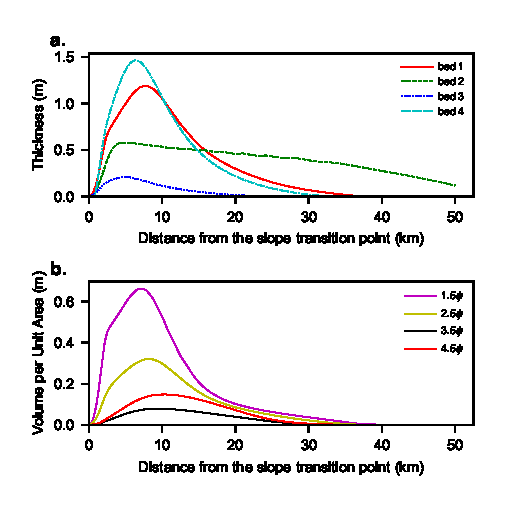
\includegraphics[width=8cm]{fig04.eps}
  \caption{Examples of turbidites calculated by the forward model. \textsf{a}. Spatial distributions of bed thickness. Four beds (Bed 1--4) were plotted as examples. \textsf{b}. Spatial distribution of the volume-per-unit-area for each grain size class in Bed 1 (Fig. 4a).}
  \label{fig:training_examples_artificial_turbidites}
\end{figure}

\subsection{Results of training}
We trained the NN inverse model with various numbers of artificial data and lengths of the sampling window, and the best result in terms of the value of the loss function for the validation sets and the practical usage of the model can be obtained with 3500 training data sets and 10 km-long sampling window  (Fig. \ref{fig:training_different_number_length}). Results with less than 2000 training data sets produce a discrepancy in the loss function between the training and the validation sets, indicating overlearning of the NN. Conversely, when the number of data sets exceeds 2000, the loss function of the validation set is slightly less than the value of the training set. As the number of training data increases, the resultant values of the loss function improve. However, when the number of data exceeds 2500, the improvement of values of the loss function became not so rapid. Regarding the distance of the sampling window, the training results are not stable when the sampling window is shorter than 5 km (Fig. \ref{fig:training_different_number_length}). On the other hand, the training results are stable when the window length is longer than 10 km, and the results gradually improve as the window length increases. However, extending the window length from 10 km to 30 km results in little improvement of the loss function. We do not fully understand why the results are not stable for sampling windows shorter than 5 km, but it probably indicates that the training results fall into a local optimum solution depending on the initial values of the weight coefficients of the neural network (given by random numbers) due to incomplete information. In any case, the loss function is very good (less than 0.01), so that even turbidites that can be tracked for less than 5 km are likely to give good results if the outcrop spacing is sufficiently narrow and detailed observation of beds is possible.

\begin{figure}[t]
  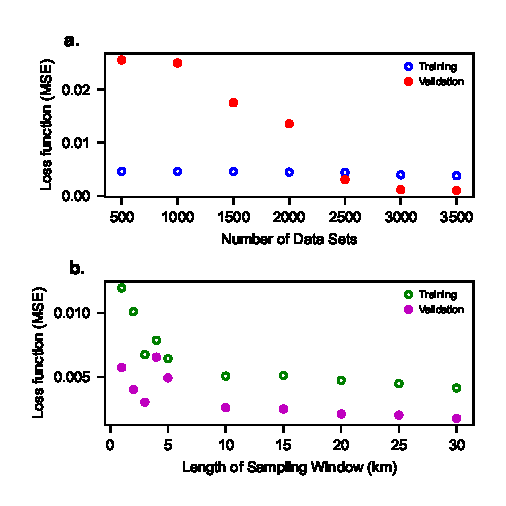
\includegraphics[width=8cm]{fig05.eps}
  \caption{Results of training of the NN with different numbers of training data sets and lengths of the sampling window.}
  \label{fig:training_different_number_length}
\end{figure}

Hereafter, we further investigate the performance of the inverse model trained on a 3500 dataset with a 10 km-long sampling window. The history of training indicates that the values of the loss function improved significantly in the first 1000 epochs, and the results are improved up to 15,000 epochs (Fig. \ref{fig:training_history}). Eventually, saturation is reached at approximately 20,000 epochs. The resultant loss function (i.e., the MSE of prediction) is $3.78 \times 10^{-3}$ for training sets and is $1.03 \times 10^{-3}$ for validation sets.

\begin{figure}[t]
  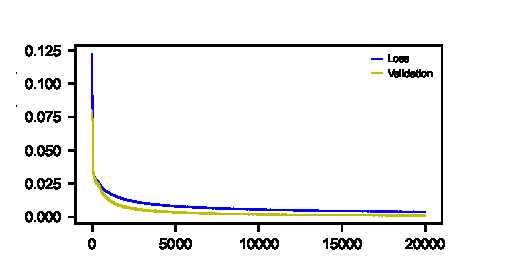
\includegraphics[width=8cm]{fig06.eps}
  \caption{Training History of the NN. 3500 datasets and 10 km-long sampling window were used for this training.}
  \label{fig:training_history}
\end{figure}


\subsection{Precision and accuracy of inverse analysis}
Using 300 test data sets, the performance of the inverse model trained with 3500 data sets and 10 km-long sampling window is evaluated. The estimated parameters are matched well with slight deviations (Figs. \ref{fig:test_scatter_plot}, \ref{fig:test_histogram_deviation}; Table \ref{table:bias_errors}). $R^2$ values are beyond 0.98 for all parameters. Particularly good agreement is obtained for the estimates of the initial height and the length of the suspended sediment cloud. Values of the normalized RMSE and MAE for these parameters are less than 9 \% and 6 \%, respectively. The sediment concentration is also precisely estimated. the normalized RMSE for the sediment concentration ranges from 12 to 16 \%, which corresponds to only 0.02--0.03 volumetric \%. The prediction for the basin slope shows relatively large errors (RMSE is close to 20 \% and MAE is 11.7 \%), but these errors correspond to only 0.03 \% of slope. Focusing on the bias of the estimates, all estimated values except for the basin slope tend to be slightly smaller, whereas the predicted values of the basin slope tend to be  larger (Fig. \ref{fig:test_histogram_deviation}). The values of the bias, however, range only from 2 to 12\% of the original value. 

\begin{figure*}[t]
  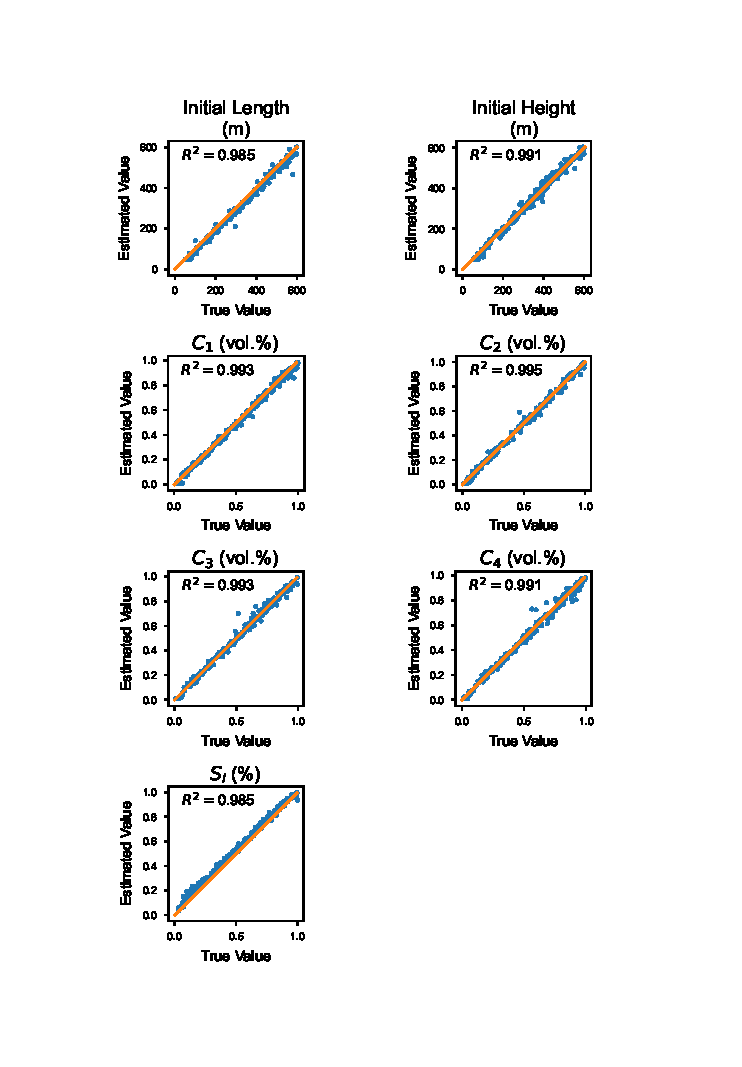
\includegraphics[width=12cm]{fig07.eps}
  \caption{Result of the inverse analysis compared with the true parameters. The x-axis represents the value of the true parameter and the y-axis represents the value of the estimated parameter. The orange lines show that the two values are in a 1:1 relationship, and thus the plots on this line indicate that the prediction is perfectly consistent with the true value.}
  \label{fig:test_scatter_plot}
\end{figure*}

\begin{figure*}[t]
  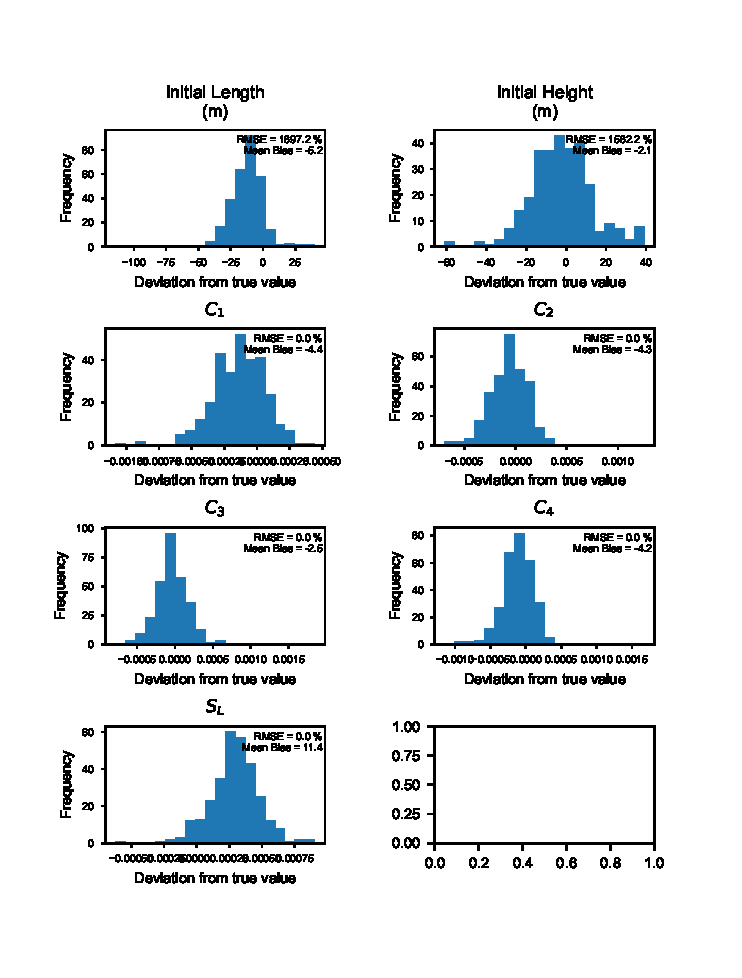
\includegraphics[width=12cm]{fig08.eps}
  \caption{Histograms indicating the deviation of the predicted values from the true values.}
  \label{fig:test_histogram_deviation}
\end{figure*}

\begin{table*}[t]
  \caption{Errors and bias of the predicted parameters. Prediction errors are exhibited by the root mean squared error (RMSE) and the mean absolute error (MAE), and the mean bias is also described. Normalized values of RMSE, MAE and mean bias by true values are also shown.}
  \begin{tabular}{lrrrrrrr}
    \hline
    {} &  $R^2$ &  RMSE &  \begin{tabular}{c} RMSE \\ (normalized) \end{tabular} &   MAE &  \begin{tabular}{c} MAE \\ (normalized) \end{tabular} &  Mean bias & \begin{tabular}{c} Mean bias \\(normalized) \end{tabular} \\
    \hline
    Initial height & 0.99 & 18.97 m &               8.55 \% & 14.81 m &              5.96 \%&     -12.93 m&                   -5.18 \%\\
Initial length & 0.99 & 15.82 m&               7.53 \%& 12.09 m&              4.92 \%&      -2.33 m&                   -2.06 \%\\
$C_1$            & 0.99 &  0.02 \%&              12.91 \%&  0.02 \%&              6.00 \%&      -0.01 \%&                   -4.44 \%\\
$C_2$            & 0.99 &  0.02 \%&              15.57 \%&  0.02 \%&              7.67 \%&      -0.01 \%&                   -4.29 \%\\
$C_3$            & 0.99 &  0.02 \%&              13.03 \%&  0.02 \%&              6.39 \%&      -0.00 \%&                   -2.49 \%\\
$C_4$            & 0.99 &  0.03 \%&              13.71 \%&  0.02 \%&              6.67 \%&      -0.01 \%&                   -4.21 \%\\
$S_l$            & 0.98 &  0.03 \%&              19.56 \%&  0.03 \%&             11.67 \%&       0.03 \%&                   11.45 \%\\
  \hline
    \end{tabular}
  \label{table:bias_errors}
\end{table*}


The forward model is calculated again using the reconstructed values to examine the influence of the estimation error of the model input parameters on the predicted flow behavior (Fig. \ref{fig:test_example_time_evolution}). The chosen test values deviate from the true conditions as indicated by the RMSE value 0.27 (Table \ref{table:example_time_evolution}), but the time evolution of the flow characteristics agree very well with those calculated from the true values (Fig. \ref{fig:test_example_time_evolution}). When comparing the velocity and concentration of the flow at 10 km from the upstream end, the discrepancy between calculation results using reconstructed and original parameters is less than 5\% for both parameters.

\begin{table*}[t]
  \caption{The predicted and the true parameters used for an example of calculation for time evolution of the flow characteristics.}
  \begin{tabular}{lrrrrrrr} \hline 
        {} &  Initial height (m) &  Initial length (m) &      $C_1$ &      $C_2$ &      $C_3$ &      $C_4$ &      $S_l$ \\
        \hline
        True input parameters &              484.41 &              318.18 &     0.17 &     0.05 &     0.95 &     0.74 &     0.23 \\
Estimated parameters  &              454.67 &              301.73 &     0.18 &     0.02 &     0.93 &     0.73 &     0.25 \\
    \hline
        \end{tabular}
  \label{table:example_time_evolution}
\end{table*}


\begin{figure}[t]
  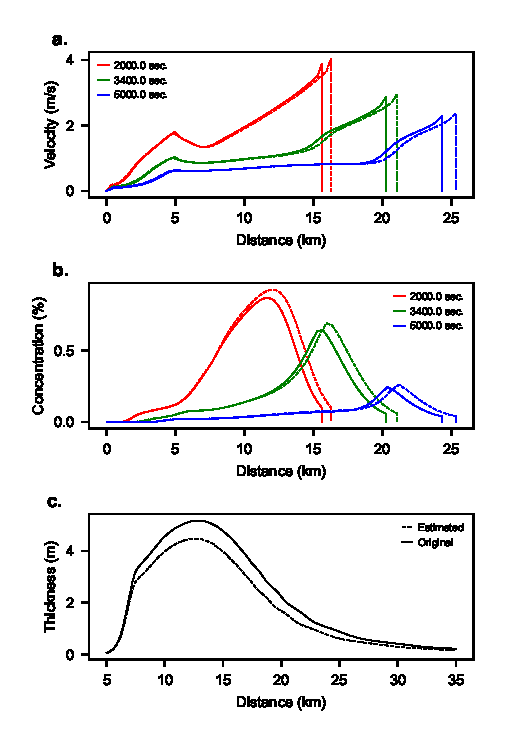
\includegraphics[width=8cm]{fig09.eps}
  \caption{Example of forward model calculation with reconstructed and true parameters. The solid line indicates the calculation result using the predicted parameters, and the dashed line exhibits the results using the true parameters. \textsf{a}. Velocity distribution at 2000, 3500 and 5000 seconds after the flow initiation. \textsf{b}. Total sediment concentration at 2000, 3500 and 5000 seconds after the flow initiation. \textsf{c}. Spatial distribution of bed thickness at 25,000 seconds after the flow initiation. }
  \label{fig:test_example_time_evolution}
\end{figure}


\subsection{Tests for robustness against noise and subsampling on input data}
The test data with various amounts of normal random values are analyzed to verify the robustness of the inverse model. Consequently, even when the standard deviation of the normal random numbers given as measurement errors was set to approximately 200\% of the value of the original data, only a small effect is observed in the normalized RMS of the results of the inverse analysis (Fig. \ref{fig:test_noise}). The RMS values gradually increase when the standard deviation of errors exceeds 50\%, but there is no rapid increase in the RMSE of the results at any particular threshold.

\begin{figure}[t]
  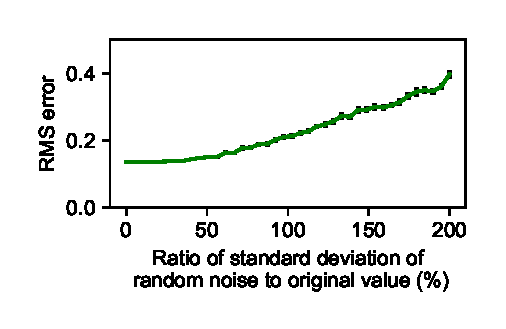
\includegraphics[width=8cm]{fig10.eps}
  \caption{Result of inverse analysis of the test data sets with artificial noise. The values of RMSE are averaged over 20 times iterations. Error bars indicate standard errors of RMSE values.}
 \label{fig:test_noise}
\end{figure}


Similarly, using subsampling data obtained by extracting some of the spatial grids from the original data, we conducted an inverse analysis of the test datasets. The results show that there is little influence on the RMSE values of the inverse analysis of the test datasets when the sampling rate of grids is greater than 1 \% (Fig. \ref{fig:test_subsampling}). The RMSE values gradually increased when the sampling rate falls below 1 \%, and RMSE becomes extremely high when the rate drops below 0.4\%.

\begin{figure}[t]
  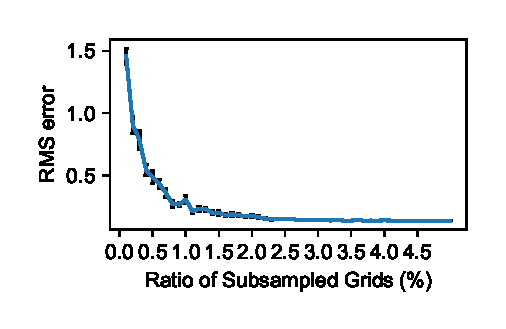
\includegraphics[width=8cm]{fig11.eps}
  \caption{Results of the inverse analysis for the subsampled test data sets. The values of RMSE are averaged over 20 times iterations. Error bars indicate standard errors of RMSE values.}
 \label{fig:test_subsampling}
\end{figure}

\subsection{Tests for influence of length of the upstream slope}
Here, a turbidite deposited in a different topographic setting was analyzed to determine the influence of the topographic assumptions to inversion results. The slope of 10 km instead of 5 km was set at the upstream end of the calculation domain. The initial conditions for this test assuming a 10 km slope were a suspended sediment cloud of 359 m high and 227 m long, with concentrations of 0.13 \%, 0.15 \%, 0.38 \%, and 0.65 \% for the four grain size classes, respectively. The gradient of the downstream slope was set to be 0.69 \%.

As a result, the initial conditions estimated by the inverse model trained on the assumption of 5 km upstream slope were a suspended sediment cloud of 117 m high and 587 m long, with concentrations of 0.33 \%, 0.38 \%, 0.48 \%, and 0.53 \% for each grain size class, and a downstream slope was estimated to be 0.96 \%. Then, these initial conditions were given to the forward model to calculate their time development, and the obtained parameters were compared on a basin plain where the turbidite was deposited (Fig. \ref{fig:test_slope_length}).

The results exhibited that the model with a 5 km slope predicted relatively close values to the original results for the flow velocity (Fig. \ref{fig:test_slope_length}). Both the model with a 5 and 10 km slope calculated velocities that were approximately 3 m/s in maximum over the basin plain and gradually decelerated downstream. However, because the slope length is different, the time to reach each point on the basin plain differs greatly.

In contrast, the concentration of the turbidity current was significantly overestimated in the model reconstruction assuming a 5 km slope (Fig. \ref{fig:test_slope_length}). When the flow reaches the downstream gentle slope at about 10 km, the original turbidity concentration was about 0.2 \% at maximum, while the restored value was closer to 0.5 \%. As a result, the thickness of turbidite estimated from the reconstructed initial values was also thicker than the original values.

\begin{figure}[t]
  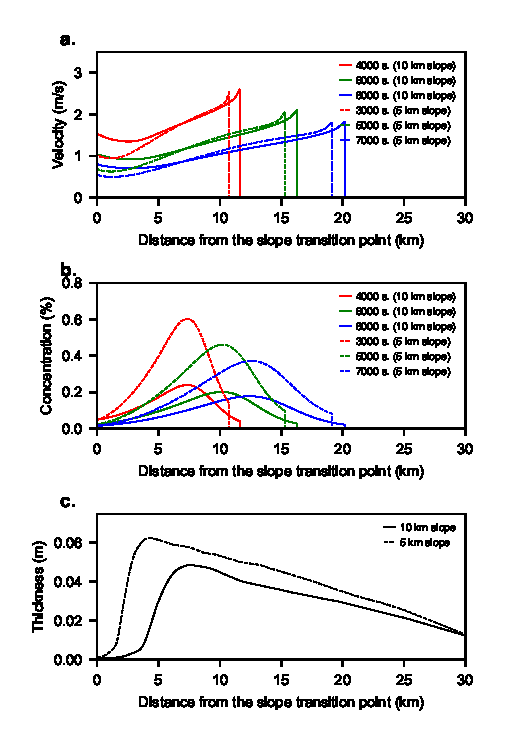
\includegraphics[width=8cm]{fig09_slope.eps}
  \caption{Influence of the length of upstream slope to the result of inverse analysis. 10 km long slope was used to produce a turbidite, and the bed was analyzed by the inverse model trained with 5 km long upstream slope. Solid lines are values for currents produced the bed, and the dashed lines are reconstructed values.  a. Time development of flow velocity. b. Total sediment concentration. c. Distribution of bed thickness.}
 \label{fig:test_slope_length}
\end{figure}




%#!pdflatex Naruse_Esurf_2020.tex
\section{Discussion}

\subsection{Performance of inverse model}
The performance of the inverse model for turbidity currents is evaluated using the test data set, implying that this model can accurately reconstruct the flow characteristics of the turbidity currents from the spatial distribution of the thickness and grain size of turbidites (Figs. \ref{fig:test_scatter_plot} and \ref{fig:test_histogram_deviation}). The biases in the values reconstructed from the true input parameters are also very small and thus should not pose a serious issue when the method is applied to actual field data.  

The inverse model not only reconstructed the initial conditions of turbidity currents accurately, but also the predicted time evolution of the flow behavior was sufficiently accurately and precisely. In the results of the forward model calculations using the predicted model input parameters that are relatively deviate from the true values (Table \ref{table:example_time_evolution}), the time evolution of the velocity and the thickness of the flow does not deviate significantly from the results using the true values (Fig. \ref{fig:test_example_time_evolution}).

Turbidity currents have a mechanism called the self-acceleration, which is caused by erosion and associated increase of the flow density \citep{parker1986self,Naruse2007,Sequeiros2009}. Therefore, even slight differences in the initial conditions of the flow can lead to very different results of the time evolution of the flow parameters. However, the results of this test imply that the accuracy of the inverse analysis in this study is enough to prevent to cause such a drastic change in the flow behavior.

The relationship between turbidity currents and characteristics of turbidites is nonlinear. Especially when the flow is self-accelerating, a small difference in the initial conditions can result in very different sedimentary characteristics. This means that it is easy to find the initial conditions of the flow by inverse analysis, because even if the characteristics of the deposits are very different, the initial conditions of the flow should not be so different. Thus, the inverse results in this case are expected to be robust even if there are some measurement errors in characteristics of deposits. In other words, there is a tradeoff between the robustness of the forward and inverse modeling.

This property of the inversion can be understood when we consider the opposite case. If the initial conditions of the flow are different but the characteristics of the turbidites are exactly the same, it is impossible to estimate the flow conditions from the turbidites. The inverse analysis of hydraulic conditions is possible because the depositional characteristics are sensitive to conditions of turbidity currents. The self-acceleration of turbidity flow is an extreme example of the sensitivity of turbidites to the flow initial conditions.

\subsection{Applicability to field-scale problems}
To apply this method to outcrops, the extent of the area that should be surveyed to collect data and the interval between outcrops should be determined. The tests with different sizes of sampling windows suggest that the survey region should be located more than 10 km from the proximal region (Fig. \ref{fig:training_different_number_length}). The loss function (i.e., the MSE of the estimates of the parameters) decreases as the length of the sampling window increases, and the best result is obtained at the 10 km-long window. Regarding the interval of the outcrops, the test results of sampling rates of more than 1.0\% with interpolation for data at non-sampled grids are not inferior to the full sample. Since the training data used in this study are computed on 5 m-spaced grids, extracting data from these grids with a 1.0\% probability is equivalent to conducting an inverse analysis from outcrop data that are distributed at 0.5 km intervals on average. Although the RMSEs of the model prediction certainly increase when the sampling rate decreases below 1.0 \%, the RMSE values does not drastically worsen until 0.5 \%. Therefore, even if the outcrop spacing is about 1 km, it should be possible to obtain a reasonable estimates of the flow characteristics.

These requirements for accurate inversion are attainable in the actual field. For example, \citet{Hirayama1977} correlated individual turbidites of the Pleistocene Otadai Formation distributed in the Boso Peninsula, Japan, on the basis of the key tuff beds. Their correlation covered a region over 30 km long with 33 outcrops. Thus, the average interval between outcrops was approximately 1 km. \citet{Amy2006} correlated individual beds in the Miocene Marnoso Arenacea Formation, Italy, using the Contessa MegaBed and an overlying ``columbine'' marker bed as the key beds. Their correlation covers 109 sections of approximately 30 m thick succession and extends over 120 km in a direction parallel to flow. Other studies in various regions (e.g., the Arnott Sandstone in France) also reported the correlation of individual turbidites in similar scale and frequency \citep{HESSE1974,Tokuhashi1979,Tokuhashi1989,Amy2000,Amy2004}. Furthermore, \citet{Bartolini1972} surveyed the Western Alboran Basin Plain, Mediterranean Sea, and discovered an individual turbidite on the sea floor at 49 cores over approximately 30 km. The records of cores in similar scale and intervals have also been reported by other studies of the modern submarine fans in different areas \citep{BORNHOLD1971, Pilkey1980}. In summary, although the method proposed in this study requires fairly high resolution data of turbidite individual beds correlated over a long distance, such conditions in ancient geological records as well as modern seafloor surveys can be achieved.

Besides these outcrop conditions, measurement errors in the field are another important factor for application. The test results suggest that the proposed inverse model of this study is very robust against random noise; random errors in the measured data have little effect on the results (Fig. \ref{fig:test_noise}). Therefore, even if localized and small-scale scouring and sedimentation occur due to some processes such as bottom currents after the deposition of a turbidite, results of inverse analysis will not be seriously affected. However, if deposits of multiple events are amalgamated to form a single thick massive sandstone, the hydraulic conditions reconstructed from the bed should be considerably different from the actual conditions. To avoid this situation, it is important to identify the erosional surface inside the bed carefully at the actual outcrop. In addition, it is safer not to analyze massive sandstones that are more than several meters thick, because they are likely to be amalgamated deposits.

Perhaps the most significant drawback to analyze actual turbidites is the assumption about the topography of the upstream submarine canyon. In this study, we tested doubling the length of the upstream slope and found that the predicted values for the concentration that were different from the original values (Fig. \ref{fig:test_slope_length}). In case of actual analysis, the upstream topography can be set correctly if the modern submarine fan is analyzed. Regarding ancient turbidites, however, some assumptions about the length and scale of the submarine canyons are necessary without measurements. In this case, it is recommended to set up various lengths of submarine canyons within a reasonable range, and to examine the degree to which these assumptions affect the inverse analysis results carefully. Nevertheless, it is worth noting that the test results were reasonable for velocity (Fig. \ref{fig:test_slope_length}), even if the assumption about the length of upstream slope was substantially different. This suggests that the inverse model proposed in this study can generally reconstruct the behavior of turbidity currents in sedimentary basins, even if the development process of turbidity currents upstream is different.


\subsection{Comparison with previous methodologies}
In existing inverse analysis methods of turbidity currents, the difference in depositional characteristics between the outputs of the forward model and the field observation is quantified as the objective function, and the initial and the boundary conditions of the forward model are determined by conducting optimization calculations to minimize the objective function \cite[e.g.,]{Nakao2017}. This is because models of turbidity currents are generally nonlinear and are difficult to linearize, especially when considering the entrainment of the basal sediment \citep{parker1986self}. Although the actual computational load depends on the choice of algorithm, this type of optimization calculation generally consists of multiple steps, and each step depends on the results of the previous calculation. Thus, the entire optimization procedure is difficult to parallelize. For instance, the kriging-based surrogate management method \citep{lesshafft2011towards} or the genetic algorithm \citep{Nakao2017} have been used to optimize the objective function for inversion of turbidity currents. In these methods, multiple calculations are conducted in each calculation step (generation), and the distribution of the objective function in the parametric space is iteratively estimated. Although the computations within each generation can be parallelized in this kind of algorithms, the next generation's computation depends on the results of the previous generation's computation, and therefore, the entire computation process cannot be parallelized. Thus, if the computational load of the forward model is high, the inverse analysis takes an unrealistic amount of time. 

\citet{Parkinson2017} applied the adjoint method with the gradient-based optimization algorithm. Although the differentiation of the layer-averaged model by the adjoint method greatly reduces the load of the gradient calculation, this approach still requires an iterative calculation for optimization. Thus, the sediment entrainment process is omitted from their model. Their model does not consider resuspension (entrainment) process of sediment, whereas suspended sand in turbidity currents is maintained by balancing the effects of particle settling and diffusion from the bottom (i.e. entrainment). Their model only considers advection and settling of particles, so that the suspended sediment quickly settles and be lost over short distances at realistic flow thicknesses and concentrations. The only way to transport large amounts of suspended sediment for long distance and to deposit thick turbidites without resuspension is to make the flow extremely thick or to suppose unusually high velocity or concentration. This is the reason for that the extremely thick flow depth (more than 3000 m) was obtained in their results. Their inversion method requires iterations that cannot be parallelized, so that the forward model needs to be simplified for this purpose. In addition, gradient-based optimization tends to have problems with initial value dependency and escaping from local optimal solutions. For this reason, the results of their inverse analysis of turbidites were quite unrealistic. In contrast, we were able to adopt "full model" that incorporate the entrainment process of suspended sand into our model without any problems. As a result, our inversion did not produce any anomalous reconstructions even though most of our test data exhibit thickness and grain size distributions similar to realistic turbidites. This strongly suggests the robustness of our inverse model and its applicability to real turbidites.

Another potential approach to optimization is the Markov Chain Monte Carlo (MCMC) method, but even with this method, repetition of the forward model calculation is unavoidable, since MCMC usually requires repetition of calculations of objective function, which cannot be parallelized, more than the order of $10^4$ time. The layer-averaged model of unsteady turbidity currents is probably not suitable for the forward models due to their computational load.

The approach proposed in this study is obviously superior to existing methods in terms of applicability to the field, as it allows computationally demanding models to be applied as forward models. The general relationship between the bed and the input parameters is learned by NN rather than adjusting the input parameters of the numerical model to reproduce the characteristics of specific individual beds. The objective function used in the training of this NN is not the difference between the features of the sediment, but the precision of the inverse analysis results themselves. The most computationally demanding part of the inverse analysis method proposed here is the generation of the training data for the NN. However, since the computations of the forward models are completely independent of each other, the generation of the training data can be conducted in parallel. Thus, our method enables us to easily prepare a large number of training data by using PC clusters, even for very computationally demanding forward models. In addition, the number of calculations required for training is not as high as other methods, specifically only approximately 3,000. It is also advantageous that the proposed method enables us to perform various tests for robustness or precision of inversion before application to field examples, because the NN outputs results of inverse analysis extremely fast. For these reasons, we consider that this study successfully generated an inverse model using the layer-averaged model for unsteady turbidity currents that can be applied to the field. 

\subsection{Limitations and future tasks}

The inverse model proposed in this study has several limitations. Inevitably, the accuracy of the inverse analysis is governed by the validity of the forward model that generates the training data. The present implementation of the inverse model uses the one dimensional layer-averaged model as the forward model, but this model is likely to be applicable only to sedimentary basins that are laterally constrained or to the inside of the submarine channels. The layer-averaged model of \citet{parker1986self} used in this study has been widely accepted, but various doubts have been recently raised such as the formulation of entrainment rates of basal sediment \citep{Dorrell2018} and ambient seawater \citep{Luchi2018}. The assumption of a lock exchange condition for the occurrence of turbidity currents may not be appropriate in some situations. 

Although \citet{Luchi2018} suggested that the a single layer model may not be sufficient for considering behavior of turbidity currents maintained over long distances, it is expected that such turbidity currents do not leave turbidites and create a bypassing zone. Otherwise, the concentration in the lower layers of turbidity currents decrease, and therefore the currents stop within a relatively short distance. Thus, a two-layer model of turbidity currents is not always necessary for inversion of bed-scale turbidites. However, modeling of continuos sustained turbidity currents is necessary for inverse analysis of the development of submarine fans and channel-levee systems in a larger scale. 

It is relatively easy to solve these problems described above. Without changing the framework of the proposed method, we can adapt to any situation by changing the forward model to generate the training data. For processes such as sediment transport, it is easy to revise the model to incorporate the state-of-the-art knowledge. By adopting computationally demanding models, inverse analysis using 2-D and 3-D forward models may be possible. In Future research, these issues should be addressed, and the methodology to actual field examples should be applied.

The analysis of ancient turbidites is an important issue in the future. However, even if ancient turbidites are analyzed, it is not possible to verify that the results obtained are correct, because the hydraulic conditions for ancient turbidity currents are unknown. Another way to verify the validity of the method is to reconstruct the hydraulic conditions of experimental turbidity currents from the turbidites deposited in the flume, and compare them with the measured values. The turbidity currents measured in the modern submarine canyons and their deposits would be another candidate to be used for the model verification.


\conclusions  %% \conclusions[modified heading if necessary]
%#pdflatex Naruse_Esurf_2020.tex

This study implemented an inverse model that reconstructs the flow characteristics of turbidity currents from their deposits using a NN, and verified its effectiveness at the field scale. In this study, we assumed that turbidity currents occur from suspended sediment clouds, which flow down from the steep slope in a submarine canyon to a gently sloping basin plain. The inverse model attempts to reconstruct seven model input parameters (height and length of the initial suspended sediment cloud, sediment concentration of four grain size classes, and slope of the basin plain) from the thickness and grain size distribution of the turbidite deposited on the basin plain. The forward model using one-dimensional layer-averaged equations was used to produce training data sets with random conditions in prescribed ranges. The NN was trained using the generated data to develop the inverse model. Thereafter, the test data generated independently from the training data were analyzed to verify the performance of the inverse model.

As a result of the training and tests conducted on the inverse model, the following was found:

\begin{enumerate}

\item More than 2000 data sets were required for the training to avoid overlearning. An increase in the number of training data sets results in improved performance of the inverse model; however, the degree of improvement becomes smaller even if more than 3000 data sets.

\item The hydraulic conditions and basin slopes were precisely reconstructed from the test data sets. The thickness and grain size distribution of the turbidites deposited over a 10 km-long interval in a sedimentary basin were sufficient to reconstruct the flow conditions.

\item The inverse model of this study is quite robust to random errors in the input data. The addition of a normal random number with about the same magnitude of the standard deviation to the original data had little effect on the results of the inverse analysis.

\item Judging from the results of subsampling tests, the inversion of turbidity currents can be performed if an individual turbidite can be correlated over 10 km at approximately 1 km intervals. 

\end{enumerate}

These results imply that the inverse model of turbidity currents proposed in this study is promising for analyzing field-scale turbidites. This method is expected to be applied to actual turbidites in the future.

%#!platex DeepLearningTurbidite.tex

\section{notation}
The symbols L, M and T denote dimensions of length, mass and time respectively. The symbol [1] denotes that the value is dimensionless.

\begin{description}
\item[$C_T$] Total layer-averaged sediment concentration [$\mathrm{1}$]
\item[$C_i$] Layer-averaged sediment concentration of the $i$th grain-size class [$\mathrm{1}$]
\item[$C_f$] Bed friction coefficient [$\mathrm{1}$]
\item[$e_{si}$] Sediment entrainment coefficient [$\mathrm{1}$]
\item[$F_i$] Volumetric fraction of the $i$th grain-size class in the active layer [$\mathrm{1}$]
\item[$L_a$] Thickness of the active layer [$\mathrm{L}$]
\item[$R$] Submerged specific density of sediment particles ($=1 - \rho_s / \rho_f$) [$\mathrm{1}$]
\item[$S$] Bed slope [1]
\item[$U$] Layer-averaged velocity of turbidity currents [$\mathrm{LT^{-1}}$]
 \item[$g$] Acceleration of gravity [$\mathrm{LT^{-2}}$]
 \item[$h$] Flow depth of turbidity current [$\mathrm{L}$]
 \item[$l_0$] Initial length of suspended sediment cloud [$\mathrm{L}$] 
  \item[$r_{0i}$] Ratio of near-bed sediment concentration of the $i$th grain-size class to layer-averaged concentration [$1$]
 \item[$t$] Time [$\mathrm{T}$]
 \item[$w_{si}$] Settling velocity of sediment of the $i$th grain-size class [$\mathrm{LT^{-1}}$]
 \item[$x$] Bed-attached streamwise coordinate [$\mathrm{L}$]
 \item[$H_0$] Initial height of suspended sediment cloud [$\mathrm{L}$] 
 \item[$J$] Number of model input parameters [1] 
 \item[$K$] Number of test datasets [1] 
 \item[$N$] Number of grain size classes [1] 
  \item[$S_l$] Basin slope [1] 
 \item[$\eta_T$] Thickness of the turbidite [$\mathrm{L}$]
 \item[$\eta_i$] Volume per unit area of sediment of the $i$th grain-size class [$\mathrm{L}$]
 \item[$\lambda_p$] Porosity of the turbidite [$\mathrm{1}$]
\item[$\rho_s$] Density of sediment particles [$\mathrm{ML^{-3}}$]
\item[$\rho_f$] Density of the water [$\mathrm{ML^{-3}}$]

\end{description}



%% The following commands are for the statements about the availability of data sets and/or software code corresponding to the manuscript.
%% It is strongly recommended to make use of these sections in case data sets and/or software code have been part of your research the article is based on.

% \codeavailability{TEXT} %% use this section when having only software code available


% \dataavailability{TEXT} %% use this section when having only data sets available


\codedataavailability{All codes and data used in this study is deposited in the respository Zenodo ()} %% use this section when having data sets and software code available


% \sampleavailability{TEXT} %% use this section when having geoscientific samples available


% \videosupplement{TEXT} %% use this section when having video supplements available


% \appendix
% \section{}    %% Appendix A

% \subsection{}     %% Appendix A1, A2, etc.


% \noappendix       %% use this to mark the end of the appendix section. Otherwise the figures might be numbered incorrectly (e.g. 10 instead of 1).

%% Regarding figures and tables in appendices, the following two options are possible depending on your general handling of figures and tables in the manuscript environment:

%% Option 1: If you sorted all figures and tables into the sections of the text, please also sort the appendix figures and appendix tables into the respective appendix sections.
%% They will be correctly named automatically.

%% Option 2: If you put all figures after the reference list, please insert appendix tables and figures after the normal tables and figures.
%% To rename them correctly to A1, A2, etc., please add the following commands in front of them:

% \appendixfigures  %% needs to be added in front of appendix figures

% \appendixtables   %% needs to be added in front of appendix tables

%% Please add \clearpage between each table and/or figure. Further guidelines on figures and tables can be found below.


\authorcontribution{HN: Conceptualization, Methodology, Software, Writing, Reviewing and Editing. KN: Software.} %% this section is mandatory


\competinginterests{All authors declare that: (i) no support, financial or otherwise, has been received from any organization that may have an interest in the submitted work; and (ii) there are no other relationships or activities that could appear to have influenced the submitted work.} %% this section is mandatory even if you declare that no competing interests are present

% \disclaimer{TEXT} %% optional section

\begin{acknowledgements}

This work was supported by JSPS KAKENHI Grant Numbers 26287127 and 20H01985. This study was also supported by the Earthquake Research Institute The University of Tokyo Joint Usage/Research Program 2018-B01.

\end{acknowledgements}




%% REFERENCES

\bibliographystyle{copernicus}
\bibliography{sedimentology.bib}


%% The reference list is compiled as follows:

% \begin{thebibliography}{}

% \bibitem[AUTHOR(YEAR)]{LABEL1}
% REFERENCE 1

% \bibitem[AUTHOR(YEAR)]{LABEL2}
% REFERENCE 2

% \end{thebibliography}

%% Since the Copernicus LaTeX package includes the BibTeX style file copernicus.bst,
%% authors experienced with BibTeX only have to include the following two lines:
%%
%% \bibliographystyle{copernicus}
%% \bibliography{example.bib}
%%
%% URLs and DOIs can be entered in your BibTeX file as:
%%
%% URL = {http://www.xyz.org/~jones/idx_g.htm}
%% DOI = {10.5194/xyz}


%% LITERATURE CITATIONS
%%
%% command                        & example result
%% \citet{jones90}|               & Jones et al. (1990)
%% \citep{jones90}|               & (Jones et al., 1990)
%% \citep{jones90,jones93}|       & (Jones et al., 1990, 1993)
%% \citep[p.~32]{jones90}|        & (Jones et al., 1990, p.~32)
%% \citep[e.g.,][]{jones90}|      & (e.g., Jones et al., 1990)
%% \citep[e.g.,][p.~32]{jones90}| & (e.g., Jones et al., 1990, p.~32)
%% \citeauthor{jones90}|          & Jones et al.
%% \citeyear{jones90}|            & 1990



%% FIGURES

%% When figures and tables are placed at the end of the MS (article in one-column style), please add \clearpage
%% between bibliography and first table and/or figure as well as between each table and/or figure.

% The figure files should be labelled correctly with Arabic numerals (e.g. fig01.jpg, fig02.png).


%% ONE-COLUMN FIGURES

%%f
%\begin{figure}[t]
%\includegraphics[width=8.3cm]{FILE NAME}
%\caption{TEXT}
%\end{figure}
%
%%% TWO-COLUMN FIGURES
%
%%f
%\begin{figure*}[t]
%\includegraphics[width=12cm]{FILE NAME}
%\caption{TEXT}
%\end{figure*}
%
%
%%% TABLES
%%%
%%% The different columns must be seperated with a & command and should
%%% end with \\ to identify the column brake.
%
%%% ONE-COLUMN TABLE
%
%%t
%\begin{table}[t]
%\caption{TEXT}
%\begin{tabular}{column = lcr}
%\tophline
%
%\middlehline
%
%\bottomhline
%\end{tabular}
%\belowtable{} % Table Footnotes
%\end{table}
%
%%% TWO-COLUMN TABLE
%
%%t
%\begin{table*}[t]
%\caption{TEXT}
%\begin{tabular}{column = lcr}
%\tophline
%
%\middlehline
%
%\bottomhline
%\end{tabular}
%\belowtable{} % Table Footnotes
%\end{table*}
%
%%% LANDSCAPE TABLE
%
%%t
%\begin{sidewaystable*}[t]
%\caption{TEXT}
%\begin{tabular}{column = lcr}
%\tophline
%
%\middlehline
%
%\bottomhline
%\end{tabular}
%\belowtable{} % Table Footnotes
%\end{sidewaystable*}
%
%
%%% MATHEMATICAL EXPRESSIONS
%
%%% All papers typeset by Copernicus Publications follow the math typesetting regulations
%%% given by the IUPAC Green Book (IUPAC: Quantities, Units and Symbols in Physical Chemistry,
%%% 2nd Edn., Blackwell Science, available at: http://old.iupac.org/publications/books/gbook/green_book_2ed.pdf, 1993).
%%%
%%% Physical quantities/variables are typeset in italic font (t for time, T for Temperature)
%%% Indices which are not defined are typeset in italic font (x, y, z, a, b, c)
%%% Items/objects which are defined are typeset in roman font (Car A, Car B)
%%% Descriptions/specifications which are defined by itself are typeset in roman font (abs, rel, ref, tot, net, ice)
%%% Abbreviations from 2 letters are typeset in roman font (RH, LAI)
%%% Vectors are identified in bold italic font using \vec{x}
%%% Matrices are identified in bold roman font
%%% Multiplication signs are typeset using the LaTeX commands \times (for vector products, grids, and exponential notations) or \cdot
%%% The character * should not be applied as mutliplication sign
%
%
%%% EQUATIONS
%
%%% Single-row equation
%
%\begin{equation}
%
%\end{equation}
%
%%% Multiline equation
%
%\begin{align}
%& 3 + 5 = 8\\
%& 3 + 5 = 8\\
%& 3 + 5 = 8
%\end{align}
%
%
%%% MATRICES
%
%\begin{matrix}
%x & y & z\\
%x & y & z\\
%x & y & z\\
%\end{matrix}
%
%
%%% ALGORITHM
%
%\begin{algorithm}
%\caption{...}
%\label{a1}
%\begin{algorithmic}
%...
%\end{algorithmic}
%\end{algorithm}
%
%
%%% CHEMICAL FORMULAS AND REACTIONS
%
%%% For formulas embedded in the text, please use \chem{}
%
%%% The reaction environment creates labels including the letter R, i.e. (R1), (R2), etc.
%
%\begin{reaction}
%%% \rightarrow should be used for normal (one-way) chemical reactions
%%% \rightleftharpoons should be used for equilibria
%%% \leftrightarrow should be used for resonance structures
%\end{reaction}
%
%
%%% PHYSICAL UNITS
%%%
%%% Please use \unit{} and apply the exponential notation


\end{document}
